\documentclass[12pt,letterpaper]{article}
\usepackage[utf8]{inputenc}
\usepackage{amsmath}
\usepackage{amsfonts}
\usepackage{amssymb}
\usepackage{fancyhdr}
\usepackage{graphicx}
\usepackage[left=0.79in, right=0.79in, top=0.79in, bottom=0.79in]{geometry}
\usepackage{listings}
\usepackage[svgnames]{xcolor}
\author{Chathan Driehuys}

\definecolor{diffstart}{named}{Grey}
\definecolor{diffincl}{named}{Green}
\definecolor{diffrem}{named}{OrangeRed}

\lstdefinelanguage{diff}{
	basicstyle=\ttfamily\small,
	morecomment=[f][\color{diffstart}]{@@},
	morecomment=[f][\color{diffincl}]{+},
	morecomment=[f][\color{diffrem}]{-},
}

\lstset{frame=tb,
	language=html,
	aboveskip=3mm,
	belowskip=3mm,
	showstringspaces=false,
	columns=flexible,
	basicstyle={\small\ttfamily},
	breaklines=true,
	breakatwhitespace=true,
	tabsize=2
}

\graphicspath{{./images/}}

\pagestyle{fancy}
\lhead{COMP 535}
\chead{SQL Injection}
\rhead{Chathan Driehuys}

\begin{document}
	\noindent \textbf{UNC Honor Pledge:} I certify that no unauthorized assistance has been received or given in the completion of this work.
	
	\vspace{.5in}
	
	\section*{Task 1}
		\begin{figure}[h!]
			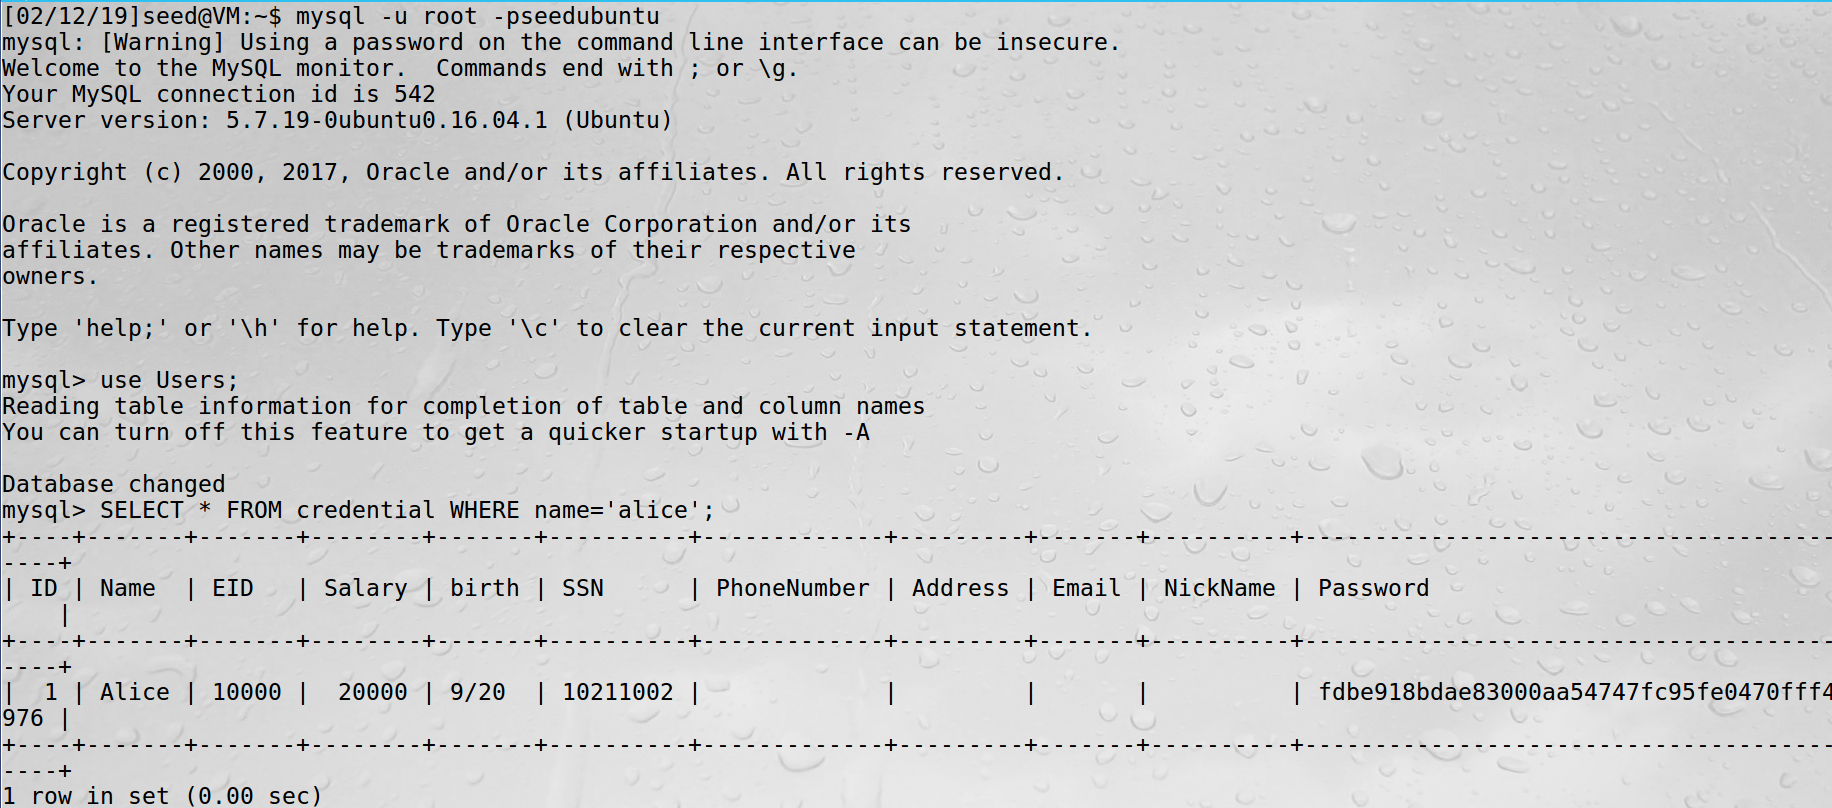
\includegraphics[width=\linewidth]{task-1-alice}
			\caption{Alice's profile information in the database.}
		\end{figure}
	
	\section*{Task 2}
		\subsection*{Task 2.1}
			We can use the username \texttt{"admin' -- "} to avoid any password validation. Note that the trailing space after the double hyphen is required for the rest of the statement to be correctly commented out.
		
			\begin{figure}[h!]
				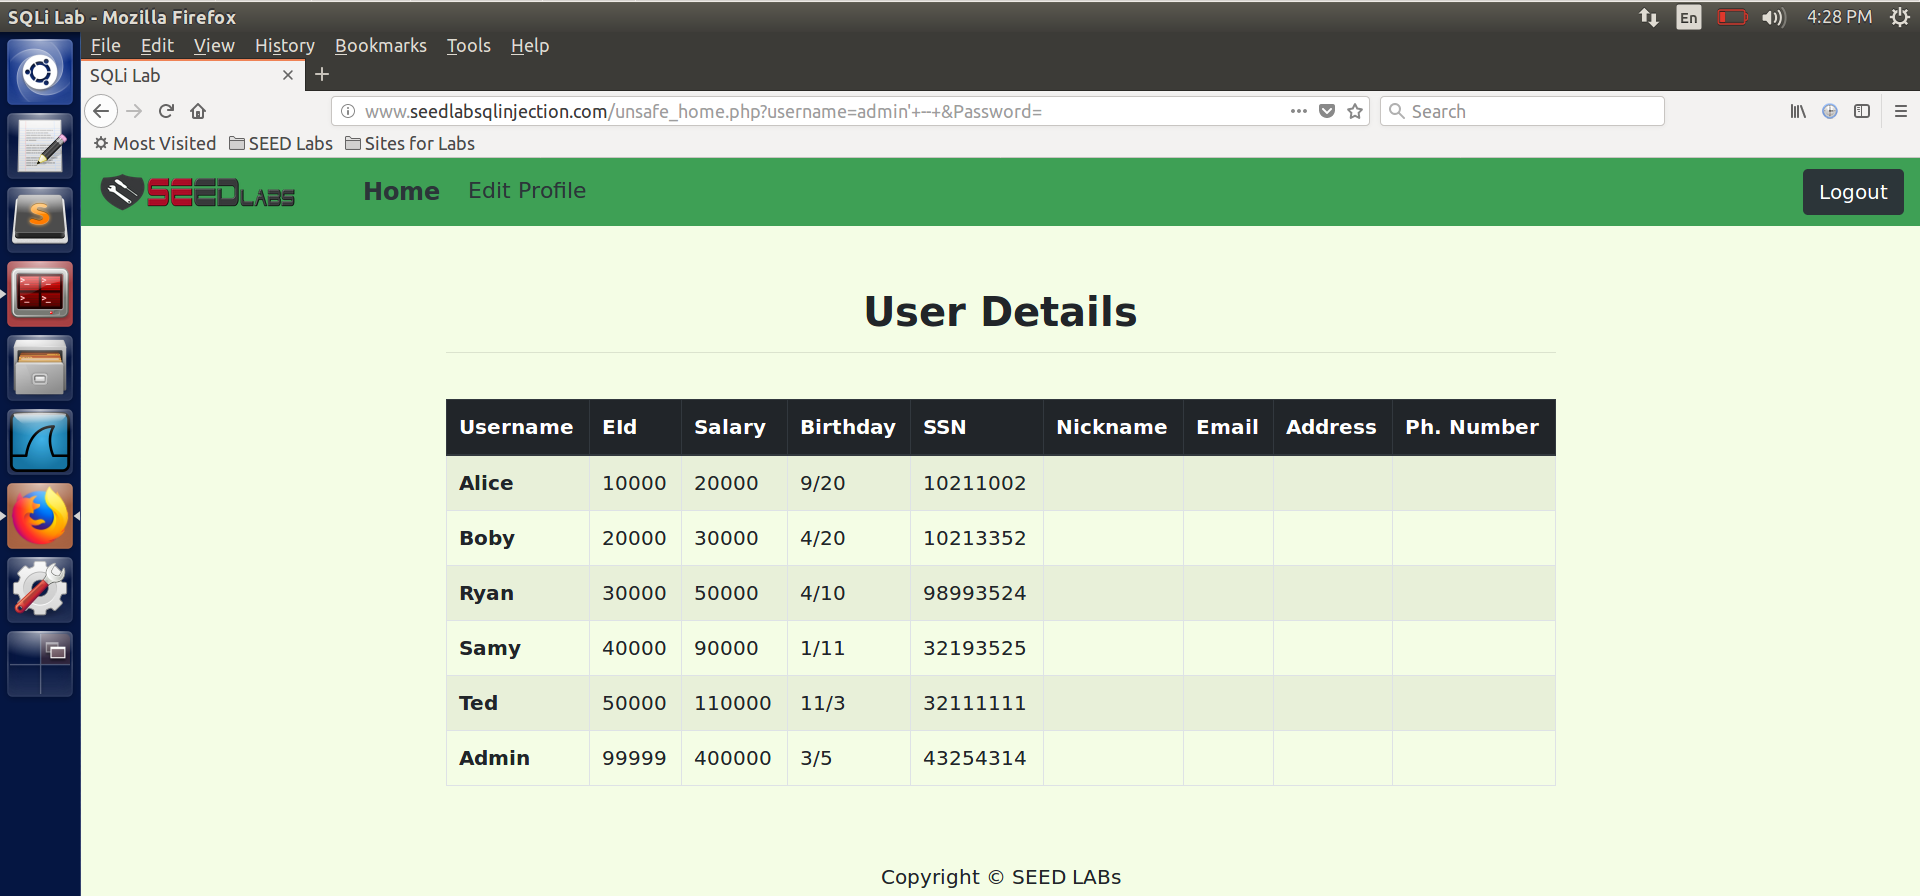
\includegraphics[width=\linewidth]{task-2-1-admin}
				\caption{Successfully gaining access to the admin view without the admin's password.}
			\end{figure}
		
		\pagebreak
		
		\subsection*{Task 2.2}
			We can perform the same injection attack from the command line by passing the username (with our injection attack) and password as \texttt{GET} parameters. The only wrinkle we have to take care of is URL encoding the spaces and other special characters used in the injection.
		
			\begin{verbatim}
				curl 'www.seedlabsqlinjection.com/unsafe_home.php?username=admin%27+--+&Password='
			\end{verbatim}
		
			\begin{figure}[h!]
				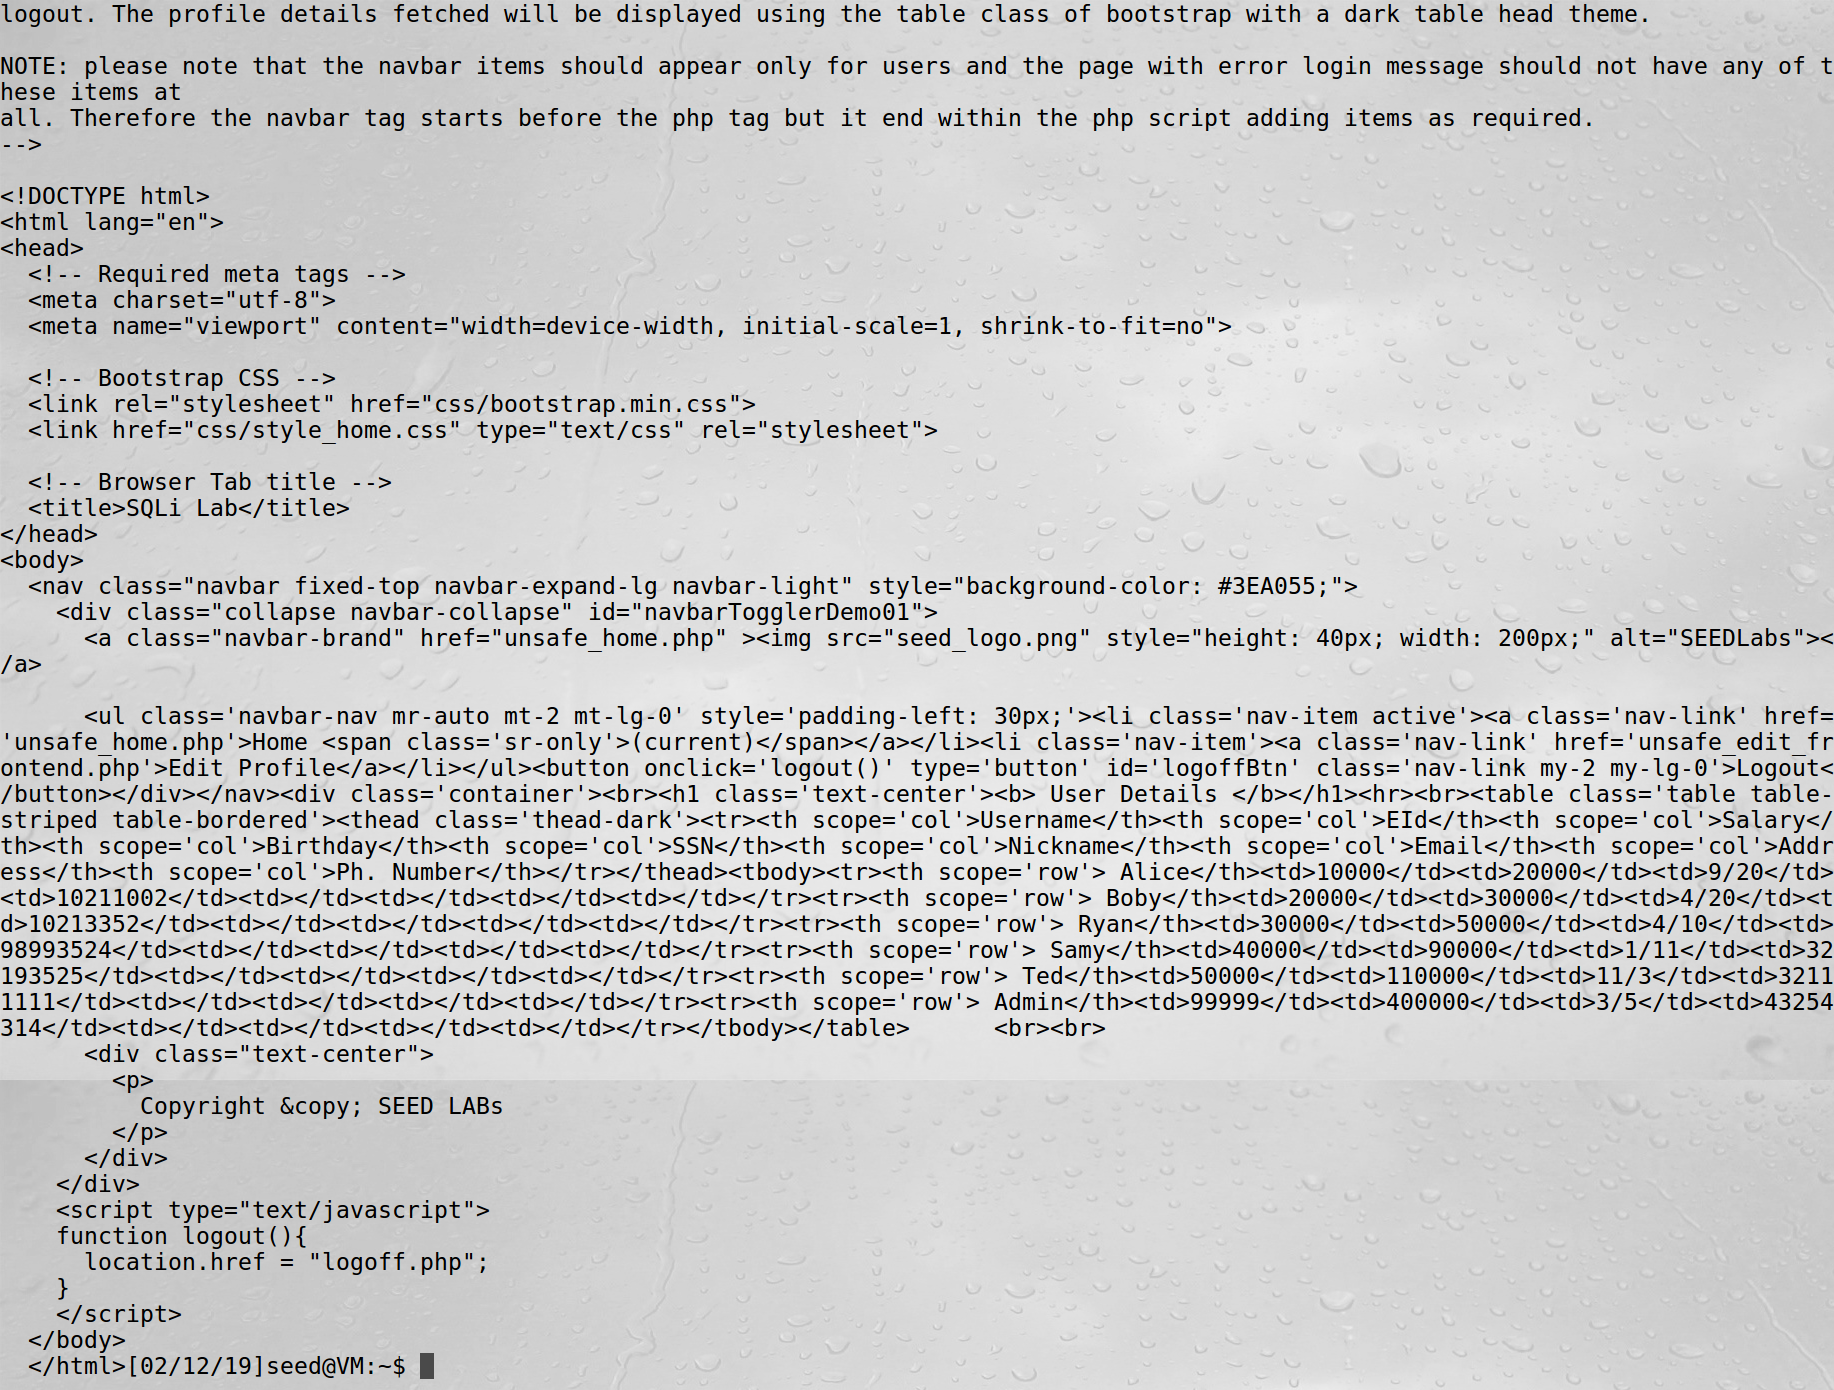
\includegraphics[width=\linewidth]{task-2-2-curl}
				\caption{The result of gaining access to the admin view from the command line.}
			\end{figure}
		
		\pagebreak
		
		\subsection*{Task 2.3}
			In order to update the database from the login page, we would have to insert something like the following into the username field:
			
			\begin{verbatim}
				admin'; UPDATE credential SET Salary=0 WHERE name='Ted'; #
			\end{verbatim}
		
			In our experiments, we could not perform multiple queries using the login page. After looking through the source code for the page and the documentation for \texttt{mysqli::query}\footnote{https://dev.mysql.com/doc/apis-php/en/apis-php-mysqli.query.html}, it appears that one cannot execute multiple statements without changing the code to use \texttt{mysqli::multi\_query}
			
	\pagebreak
			
	\section*{Task 3}
		\subsection*{Task 3.1}
			If Alice logs in, navigates to the ``Edit Profile'' page, places the following statement in the ``NickName'' field, and submits the form, she can successfully change her salary.
			
			\begin{verbatim}
			Alice', Salary=1000000 WHERE name='alice'; #
			\end{verbatim}
			
			\begin{figure}[h!]
				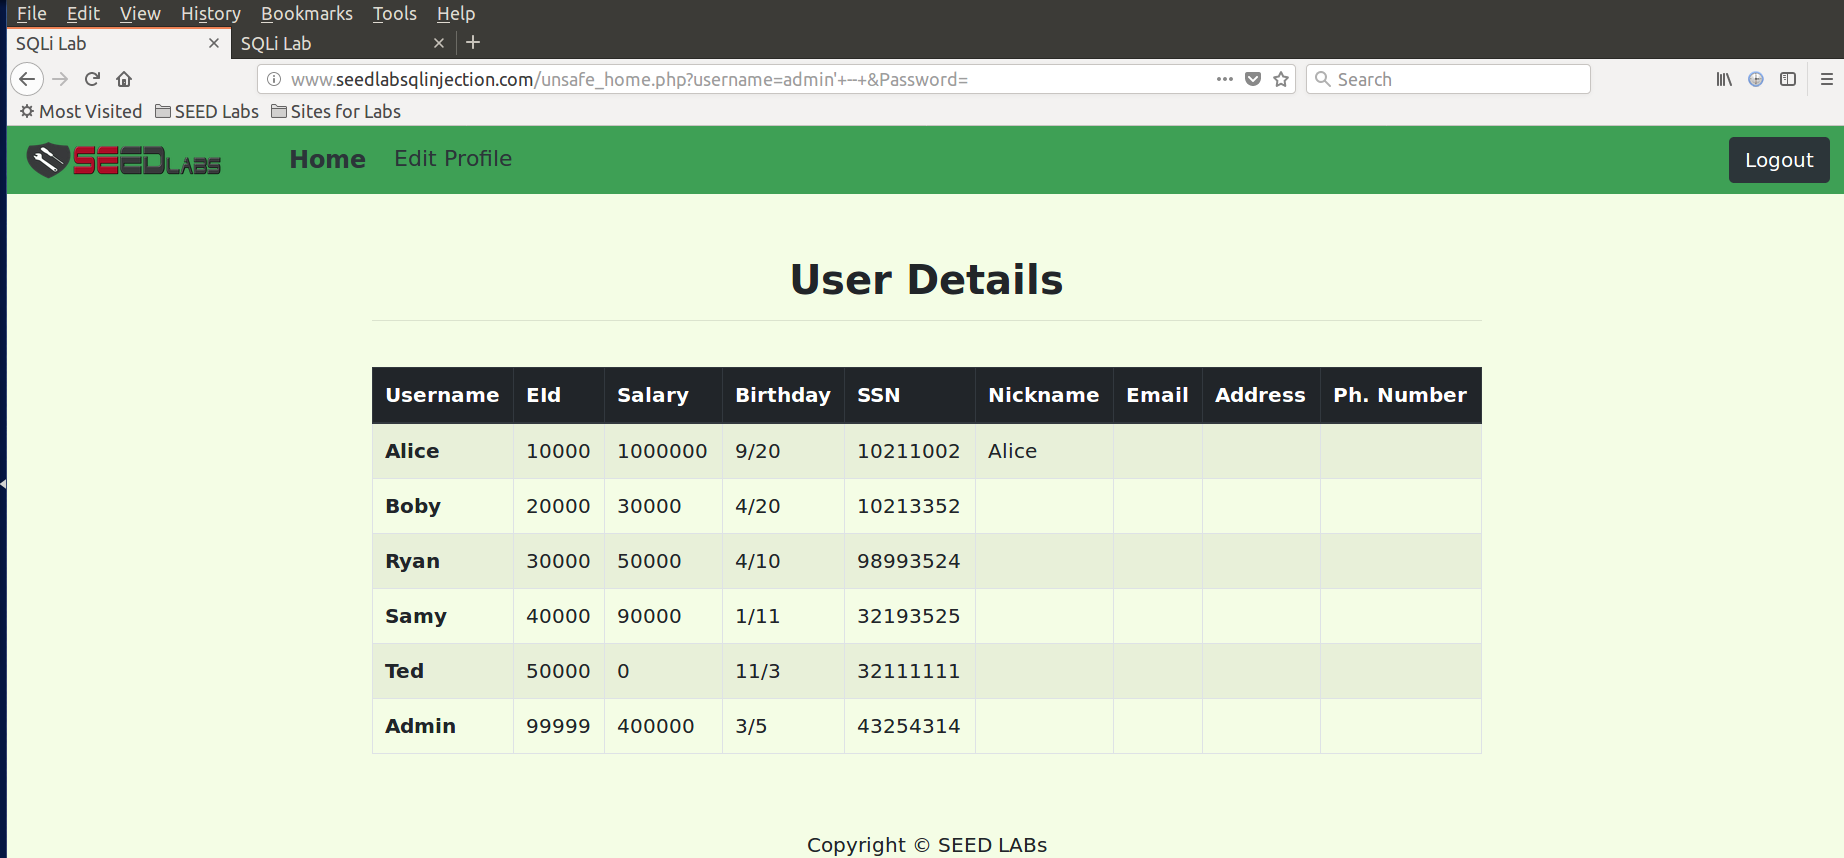
\includegraphics[width=\linewidth]{task-3-1-admin}
				\caption{The admin view now shows Alice's ``updated'' salary.}
			\end{figure}
		
		\subsection*{Task 3.2}
			To modify the profile of someone else, we can modify our statement from the previous task to target a different name. To target Boby, we would insert the following statement into the ``NickName'' field.
			
			\begin{verbatim}
			', Salary=1 WHERE name='boby'; #
			\end{verbatim}
			
			\begin{figure}[h!]
				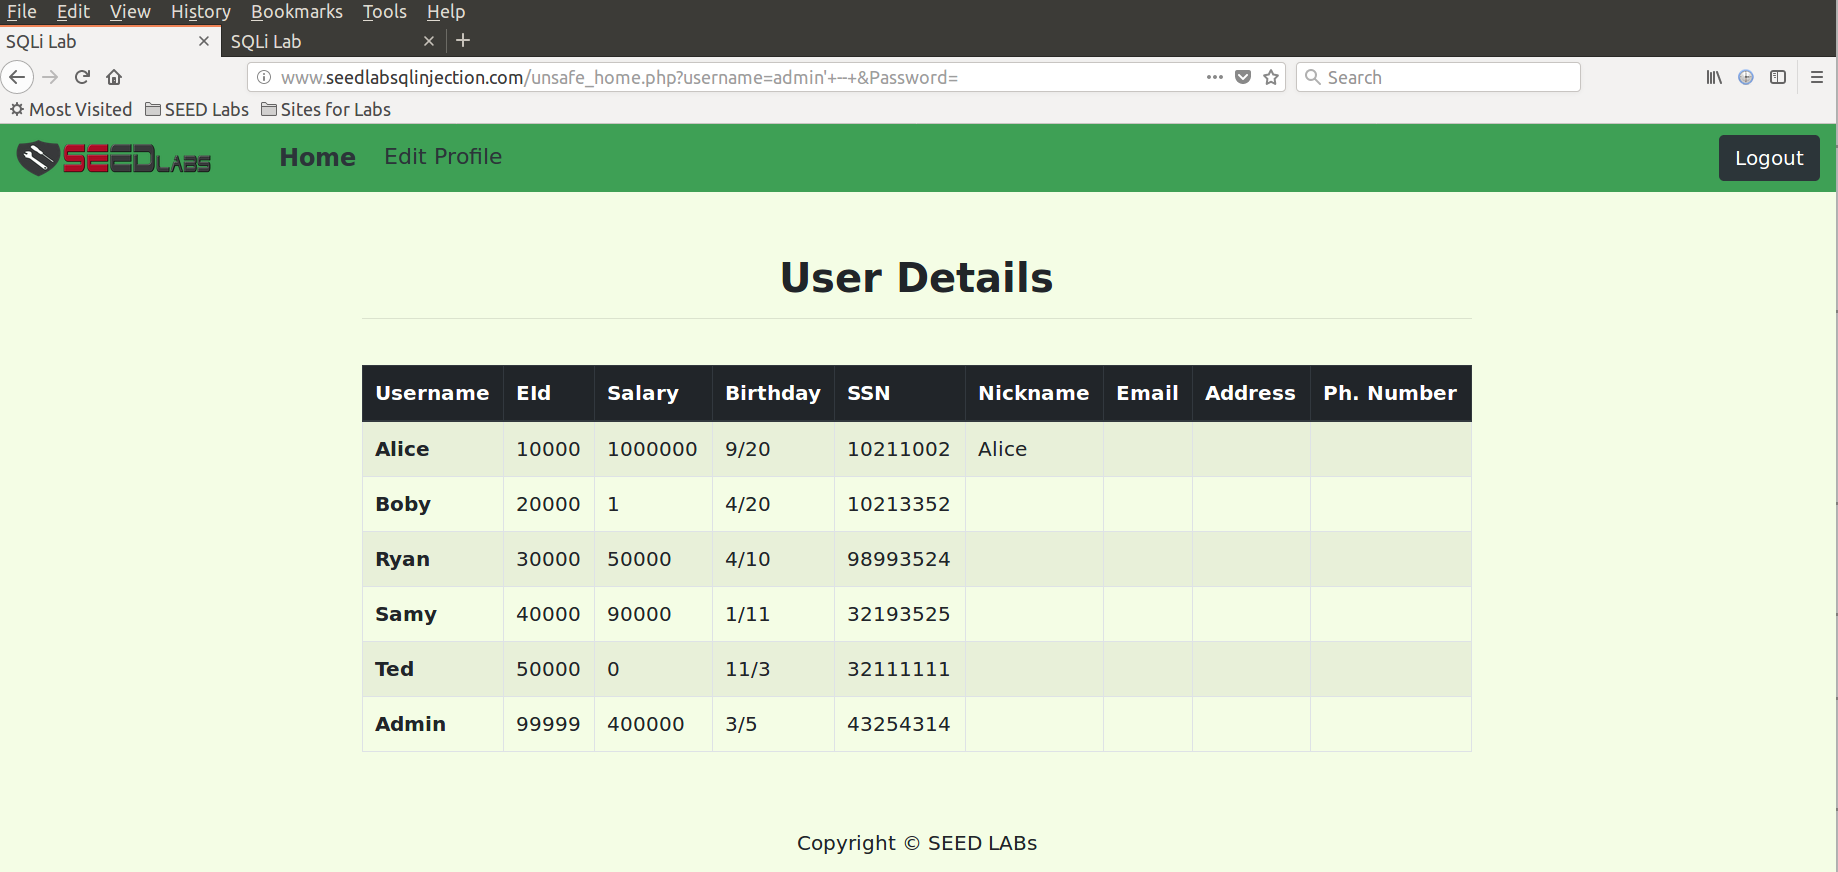
\includegraphics[width=\linewidth]{task-3-2-admin}
				\caption{The admin view now shows Boby's ``updated'' salary.}
			\end{figure}\textsf{\textsf{\textsf{}}}
		
		\pagebreak
		
		\subsection*{Task 3.3}
			This task is slightly different because we need to insert a real value into the password input because the backend hashes that value and sets it as the new password. Since the executed query updates the password field and then the phone number field, we can pass our new password into the password field and handle the injection to target Boby in the phone number input.
			
			If we input \texttt{password} into the ``Password'' field and insert the following statement into the ``Phone Number'' field, we can change Boby's password to \texttt{password}.
			
			\begin{verbatim}
			' WHERE name='boby' #
			\end{verbatim}
			
			If we open up the database console, we can see that Boby's password is now the SHA1 hash of \texttt{password}.
			
			\begin{verbatim}
			mysql> SELECT name, password FROM credential WHERE name='boby';
			+------+------------------------------------------+
			| name | password                                 |
			+------+------------------------------------------+
			| Boby | 5baa61e4c9b93f3f0682250b6cf8331b7ee68fd8 |
			+------+------------------------------------------+
			\end{verbatim}
			
	\section*{Task 4}
		\subsection*{Home Page}
			For the home page, the one vulnerable query is the one that looks up a user's profile using their username and hashed password. If we convert this part of the file to use prepared statements, all our previous attacks against the login page are mitigated.
			
			Additionally, converting to prepared statements allows us to clean up the implementation for fetching the data from the database and converting it into a format we can work with.
			
			\lstinputlisting[
			    caption={The diff of the changes needed to make the original \texttt{unsafe\_home.php} file safe.},
			    language=diff
			]{../home.diff}
		
		\subsection*{Edit Page}
			The profile edit page requires two prepared queries, one for the case where a new password is provided and one for when no new password is given.
			
			\lstinputlisting[
			    caption={The diff of the changes needed to make the original \texttt{unsafe\_edit\_backend.php} file save.},
			    language=diff
			]{../edit_backend.diff}
			
			\begin{figure}[h!]
				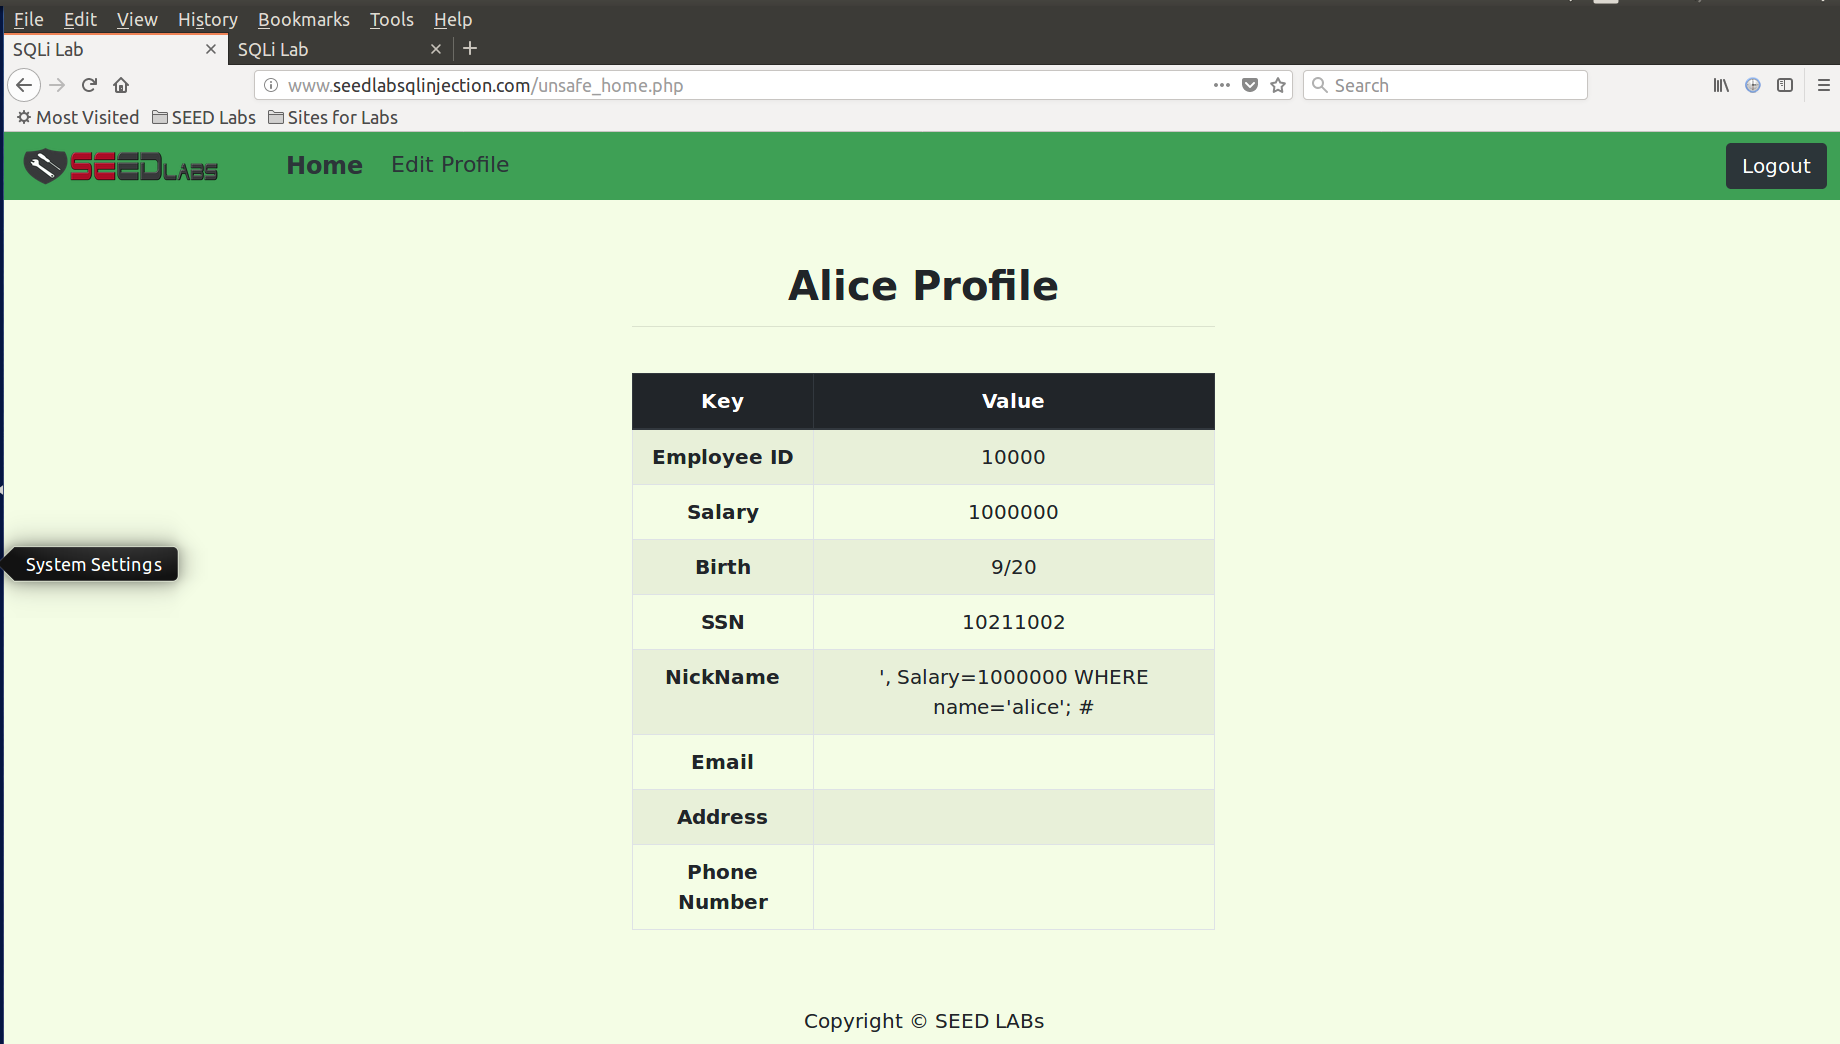
\includegraphics[width=\linewidth]{task-4-example}
				\caption{An example of SQL injections no longer working when editing the profile. The full injection string is simply saved to the field.}
			\end{figure}
		
\end{document}